\newpage

\chapter{Definitions, Clarifications and Explanations}

\label{ch:defs}

\section{Chapter \ref{ch:concept}}

\subsection*{Definitions}

\label{sec:defs3}

\textbf{Platform}: A solution neutral reference to the system that is being conceptualised. Used interchangeably with \acf{nsoi}, the platform has defined boundaries and interfaces with the \acf{wsoi} and the environment.

\textbf{User}: Refers to the cyclist who will be using the developed platform. At this stage, conceptualisation was focused on the development of the platform as opposed to the overarching objective of providing source material and resources to future development.

\subsection*{Explanations}

\subsubsection{Performance Requirements \ref{PR:27speed} \& \ref{PR:29speed}:}

The typical speed of a cyclist typically ranges from \SI{10}{\kilo\meter\per\hour} to \SI{50}{\kilo\meter\per\hour} when cycling on reasonably flat ground. For the design of the platform, a speed of maximum required speed of \SI{50}{\kilo\meter\per\hour} was assumed. Considering the two wheel sizes that were identified in Section~\ref{sec:specs}, the expected wheel rotational speeds are determined by Equation~\ref{eq:omega}.

\begin{equation}
	\ac{omega} = \frac{2 \ac{v}}{D_{wheel}}
	\label{eq:omega}
\end{equation}

\subsubsection{Performance Requirement \ref{PR:power}:}

Typically, amateur cyclists maintain an average power output between \SI{75}{\watt} and \SI{280}{\watt}, and pro cyclists can maintain up to \SI{400}{\watt}, during a 1 hour workout. As the cyclist's speed increases, less torque is required to maintain the same power output. The relation is expressed as Equation~\ref{eq:pow} and can be used to determine the force that would need to be applied at different wheel speeds to achieve these power outputs.

\begin{figure}[H]
	\begin{center}
		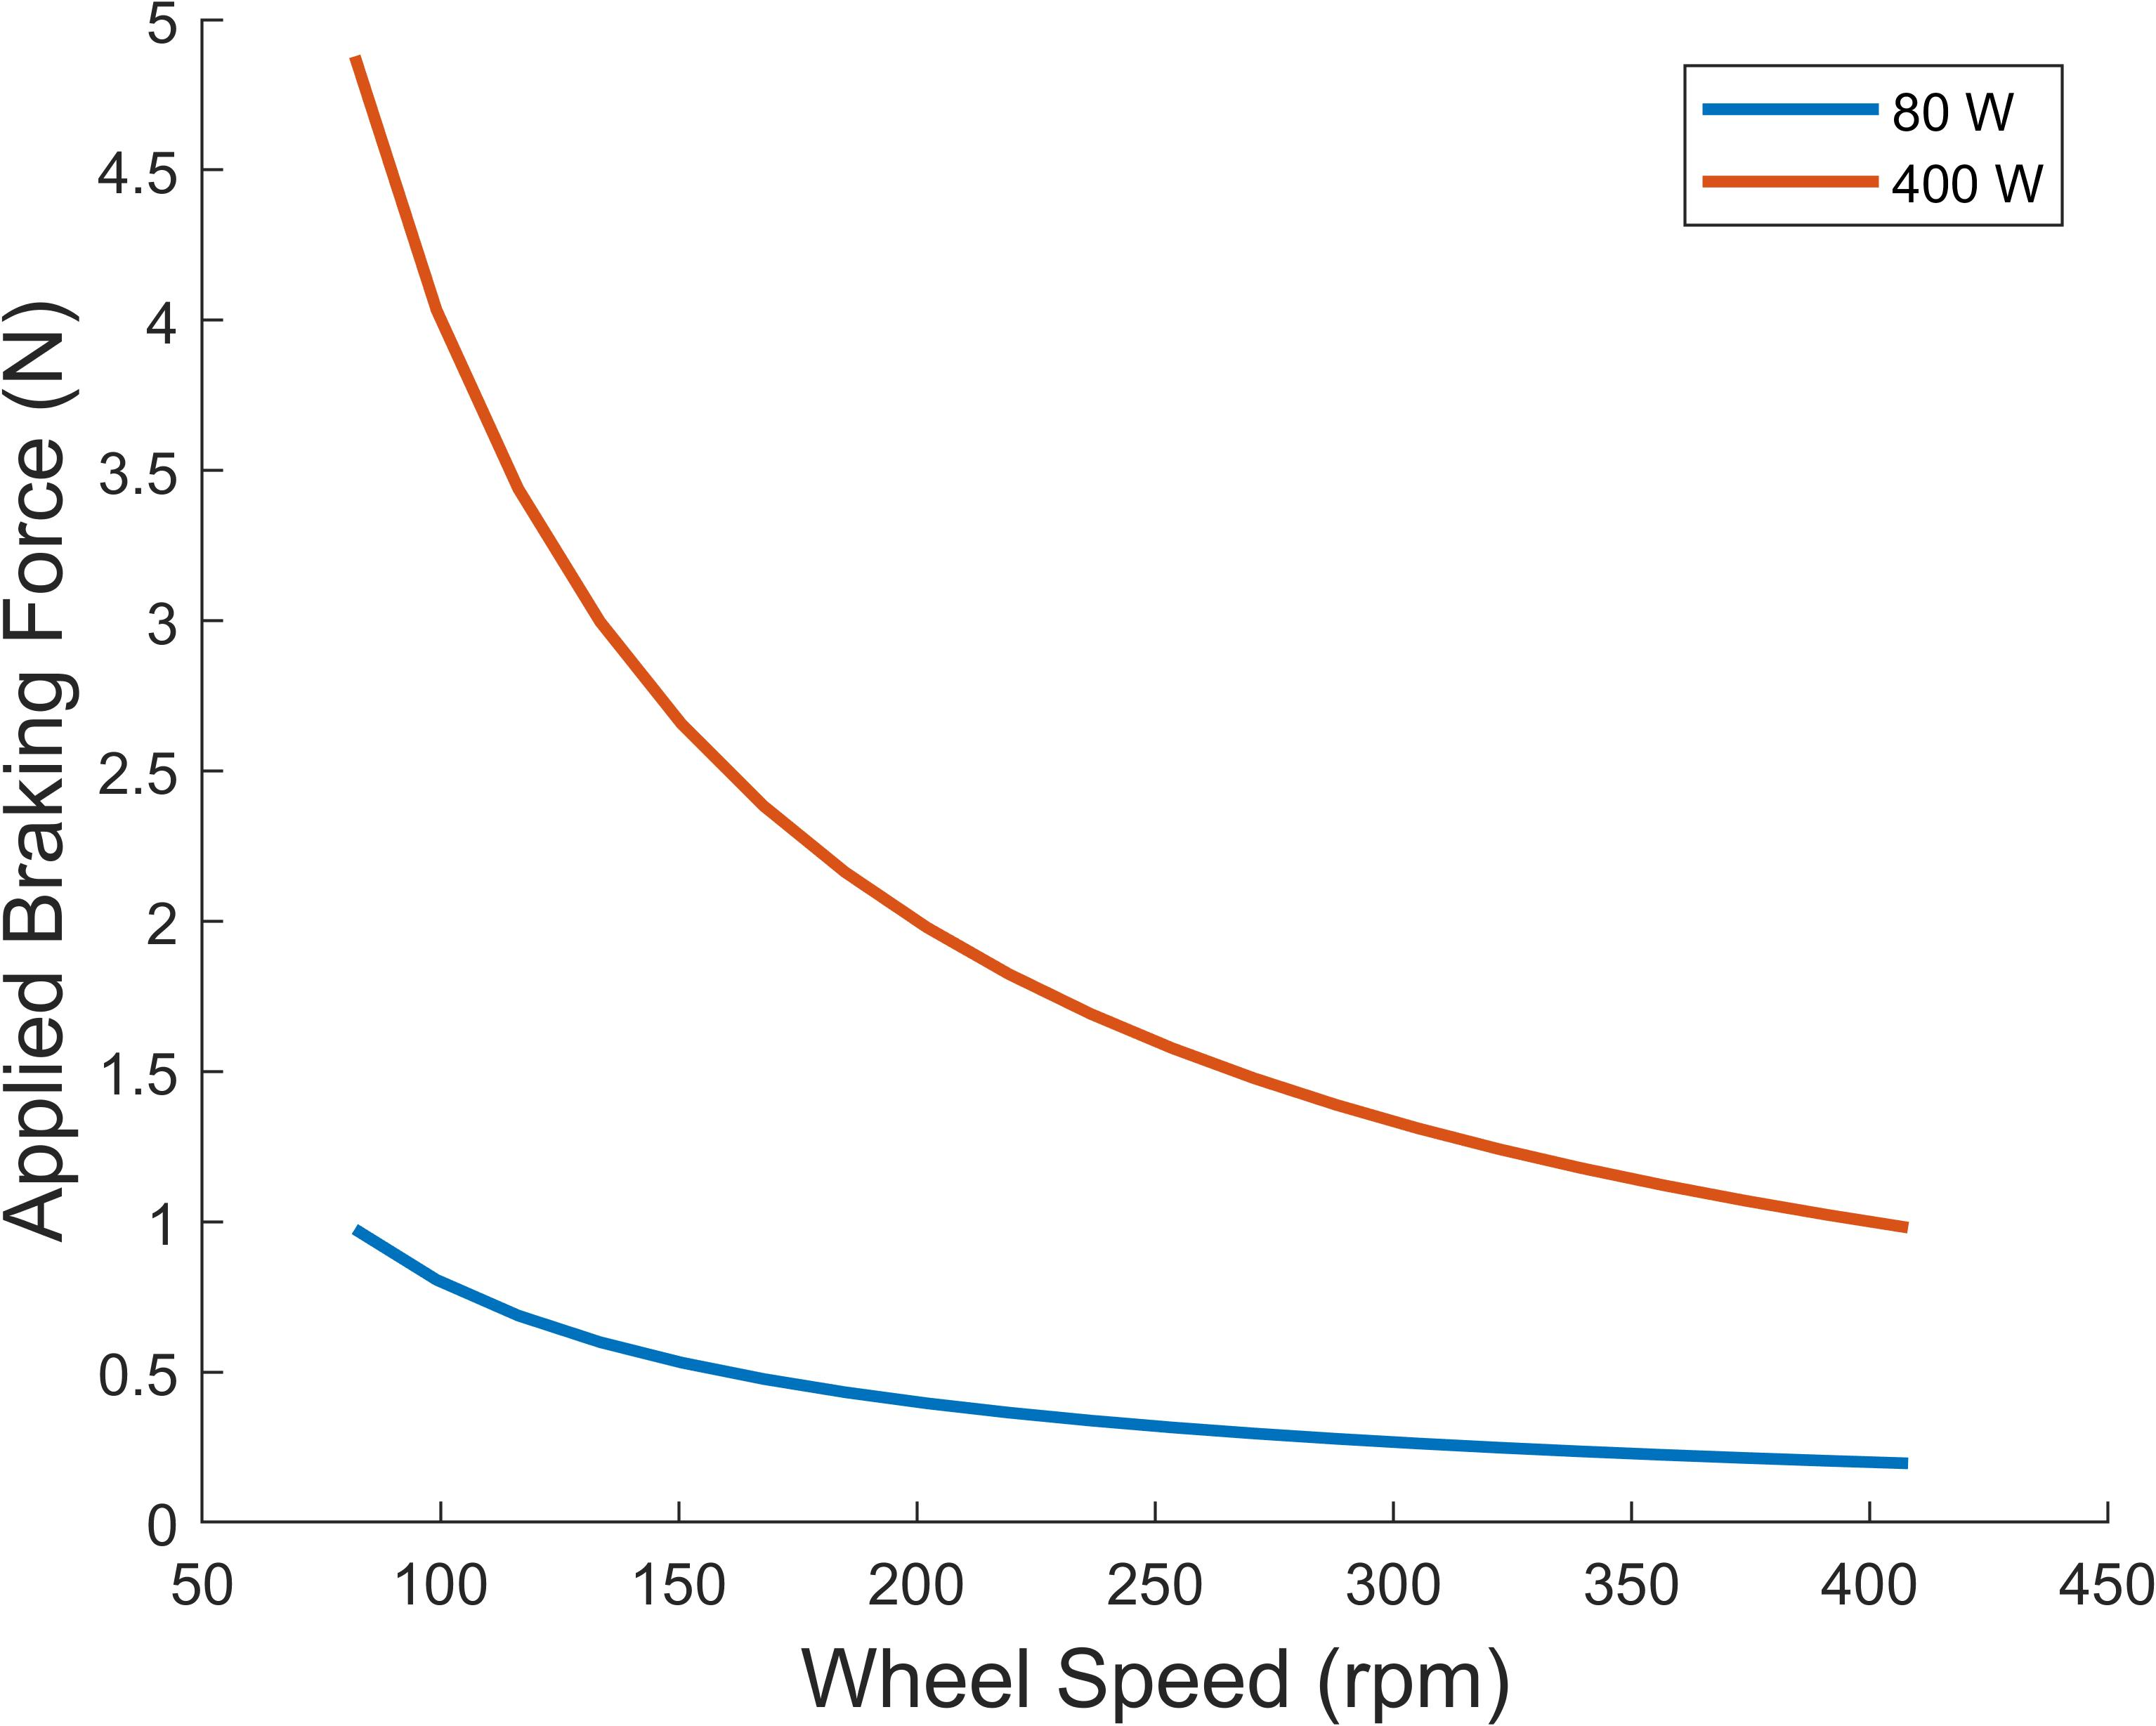
\includegraphics[width=0.65\textwidth]{BrakingForce.jpg}
		\caption{Required Braking Force Range}
		\label{fig:force}
	\end{center}
\end{figure}

\subsubsection{System Interface 2: \ac{ble} with \ac{ftms} implementation}

In order to achieve Design Objective 3, requiring the development of software that will be usable by future projects, dependency on the Zwift application \ac{api} had to be avoided. This resulted in the development of software that will enable micro controllers to interact with application hosts in a similar way to conventional smart trainers. This means that the solution will be compatible with the Zwift application irrespective of the device that acts as a host for the application. \ac{ble} was chosen as the communication protocol as this is what is available on most consumer electronic devices that Zwift is expected to operate on, and will thus not need an external unit to communicate with the platform.

%\begin{figure}[h!]
%	\centering
%	\begin{subfigure}[b]{.475\textwidth}
	%		\centering
	%		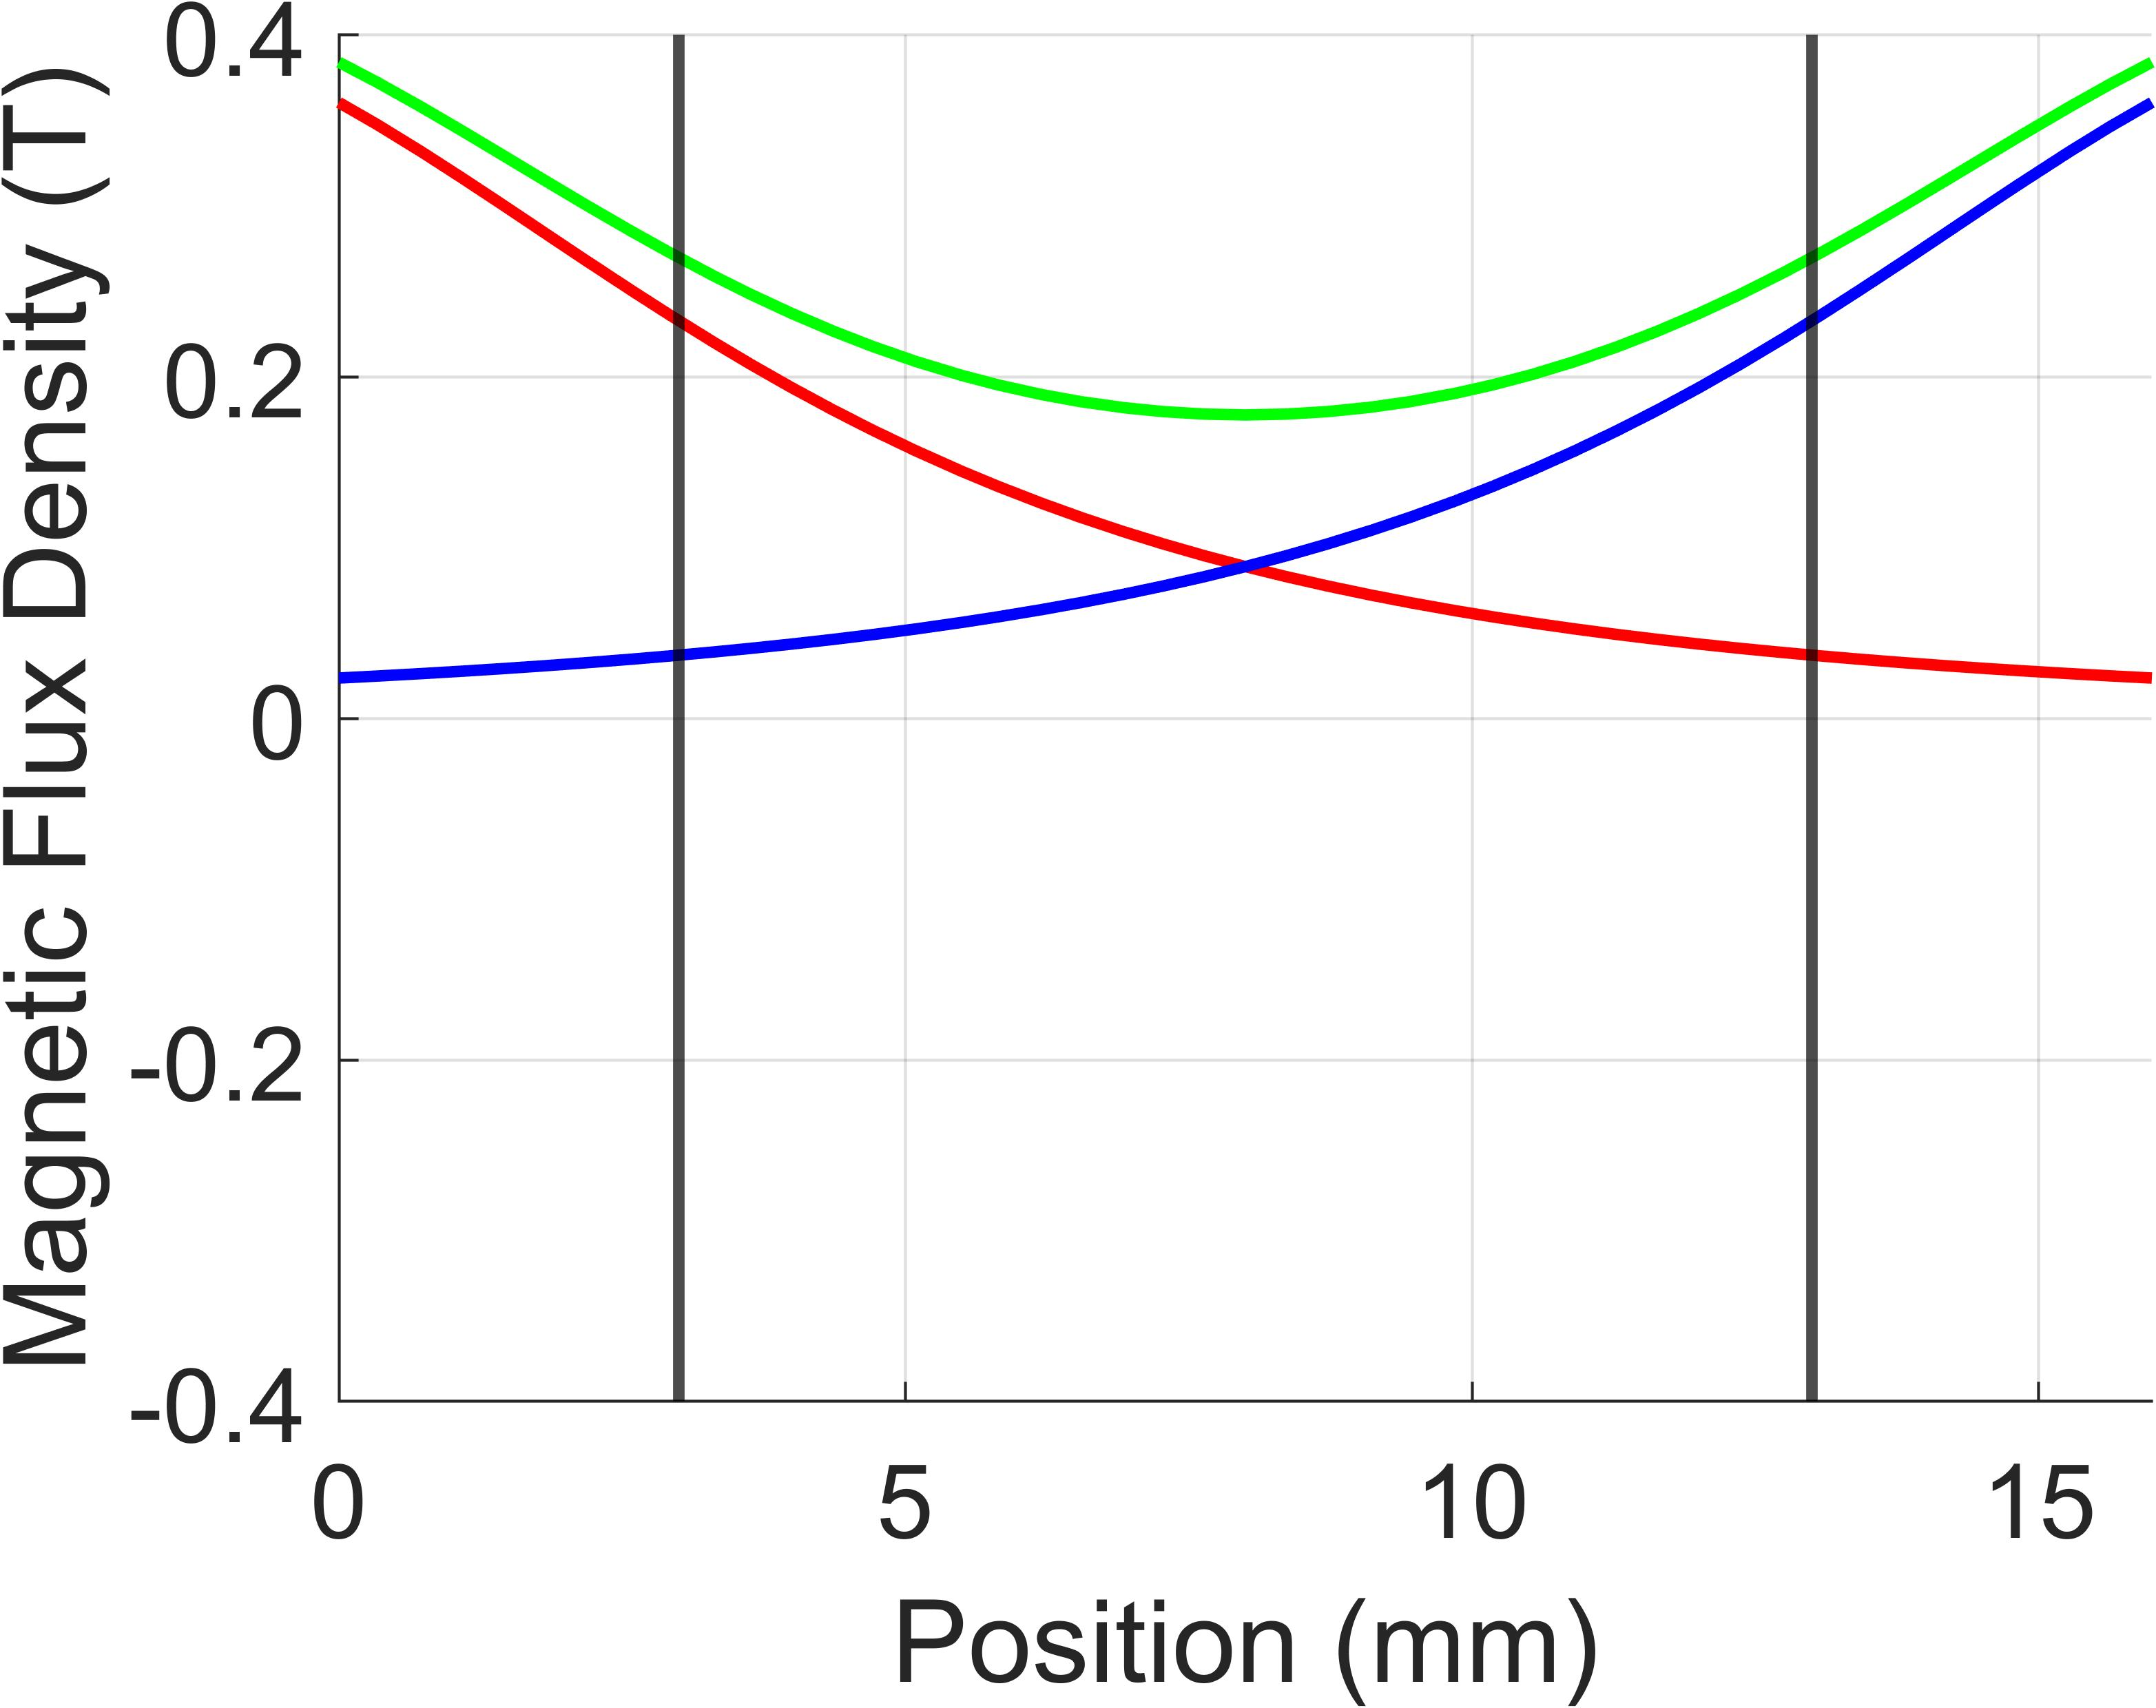
\includegraphics[width=.9\linewidth]{FluxZeroDeg.jpg}
	%		\caption{\SI{0}{\degree} Phase}
	%		\label{fig:Flux0}
	%	\end{subfigure}
%	\hfill
%	\begin{subfigure}[b]{.475\textwidth}
	%		\centering
	%		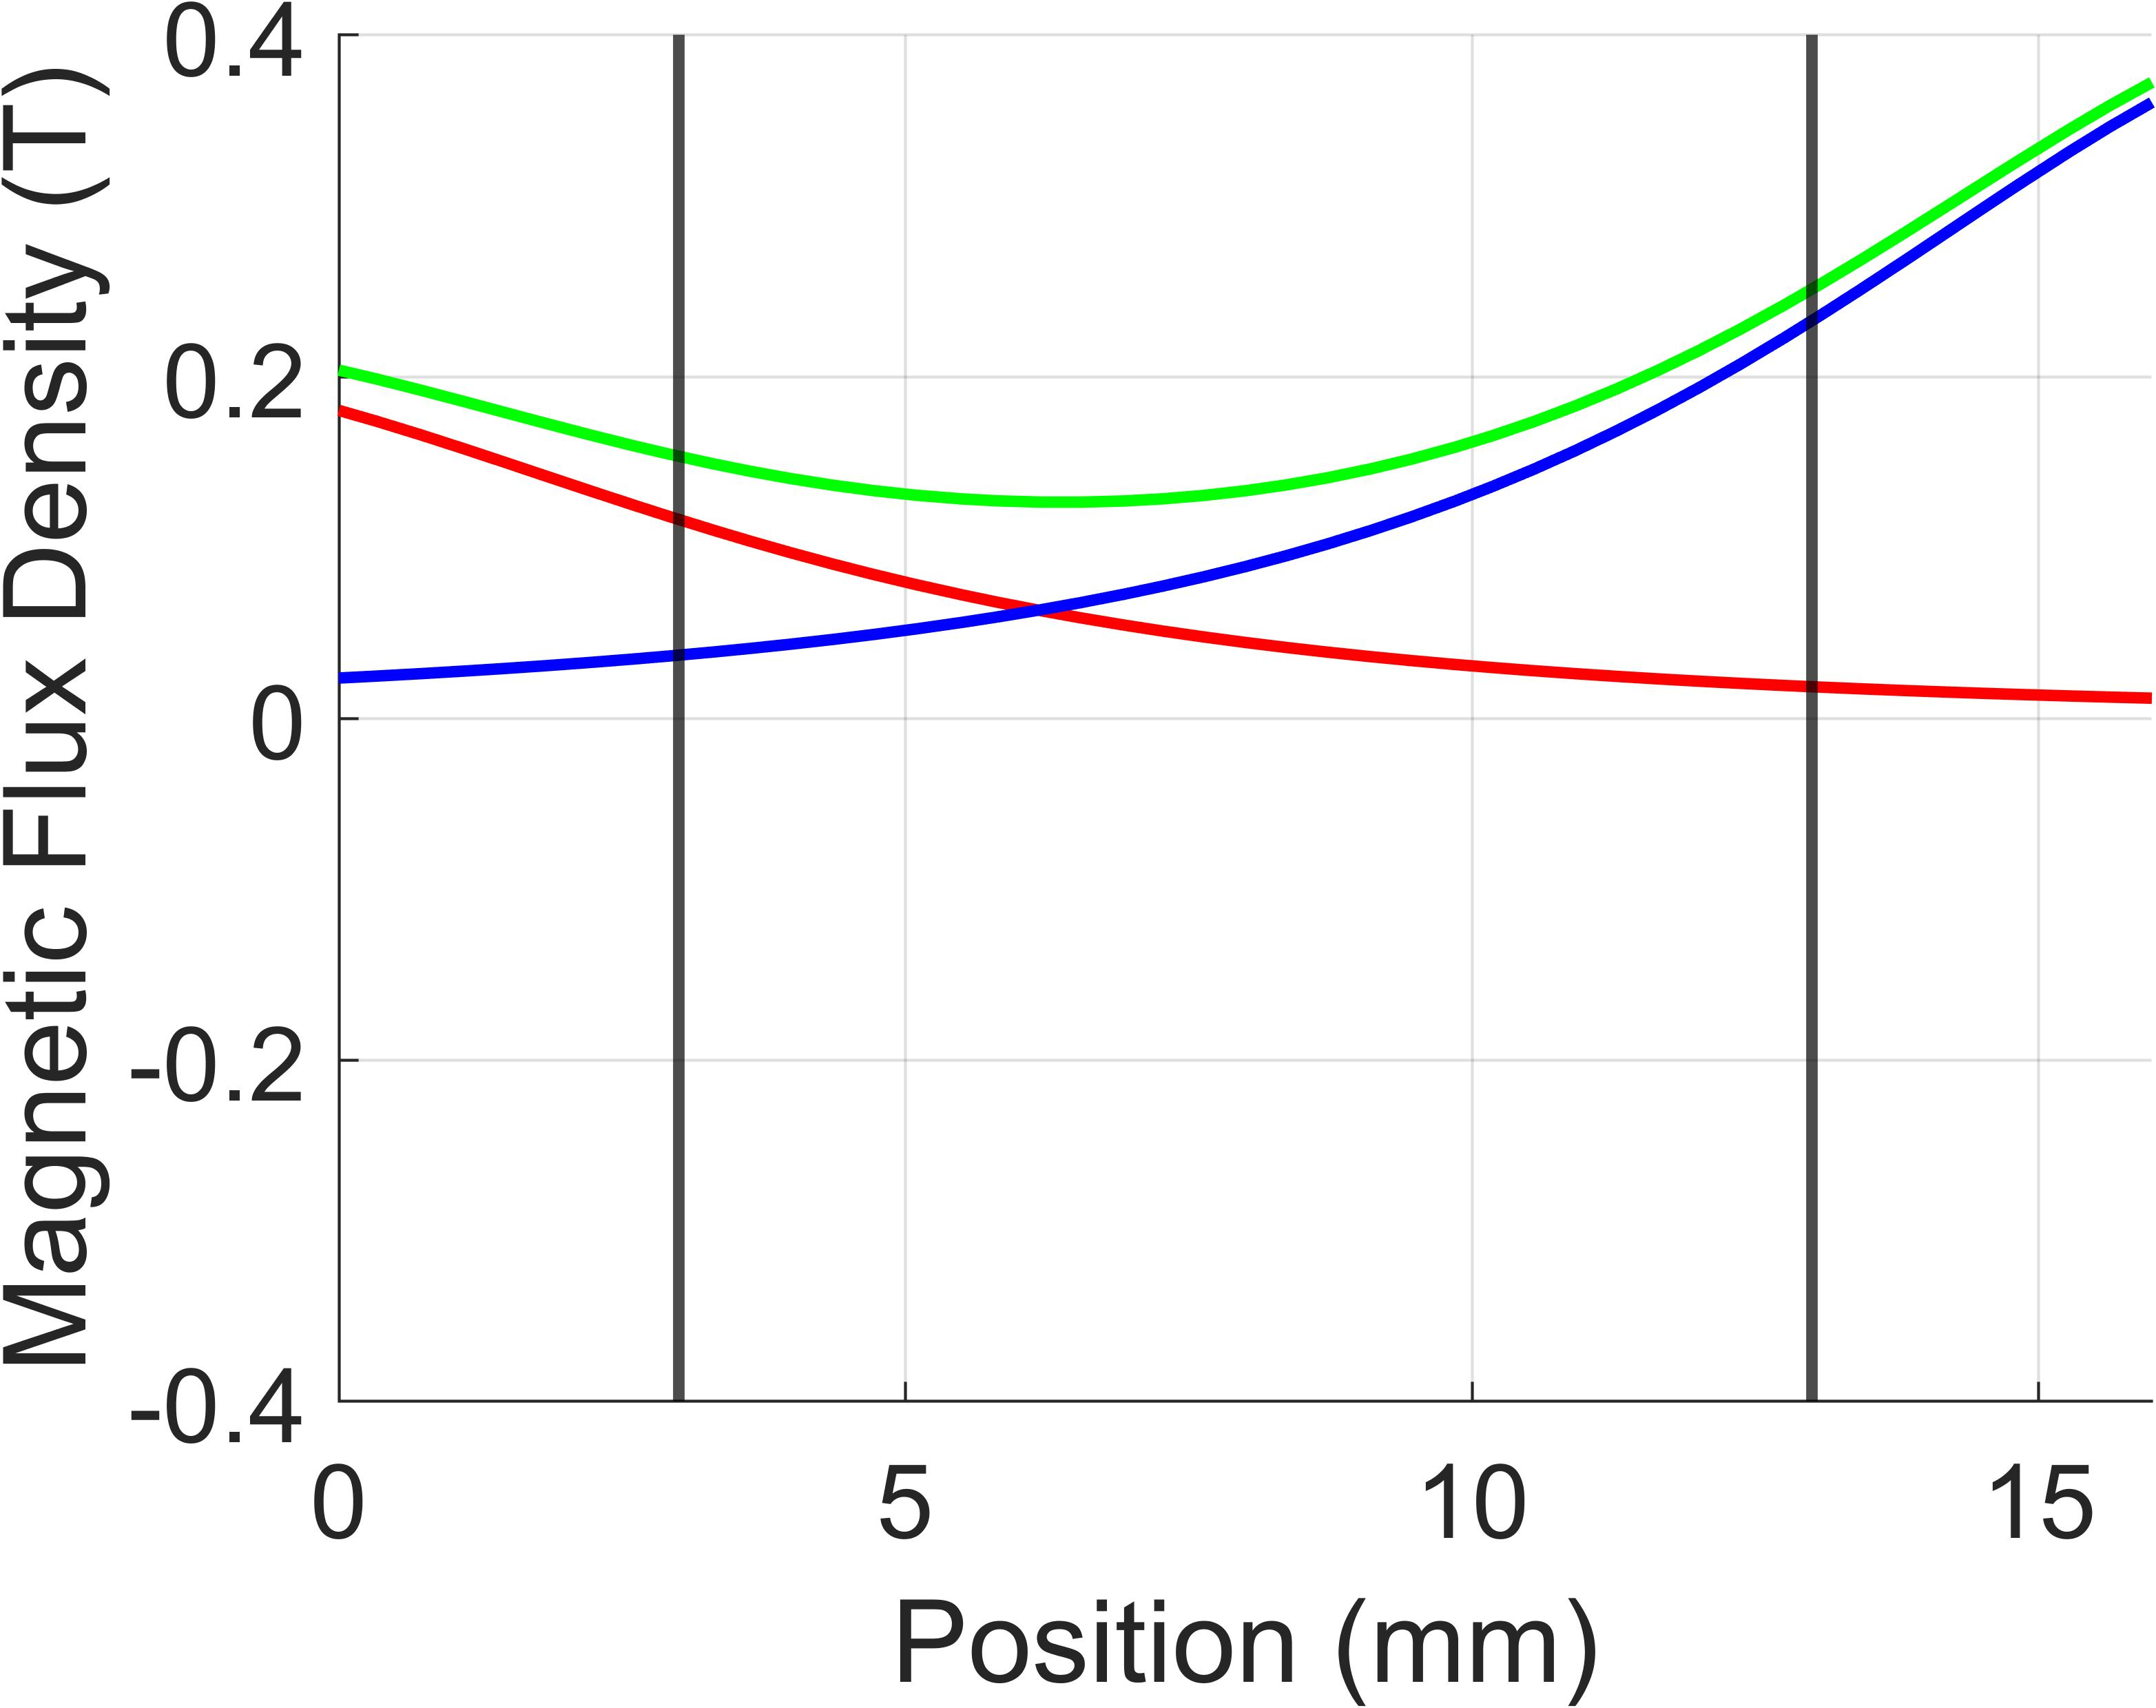
\includegraphics[width=.9\linewidth]{FluxSixtyDeg.jpg}
	%		\caption{\SI{60}{\degree} Phase}
	%		\label{fig:Flux60}
	%	\end{subfigure}
%	\vskip\baselineskip
%	\begin{subfigure}[b]{.475\textwidth}
	%		\centering
	%		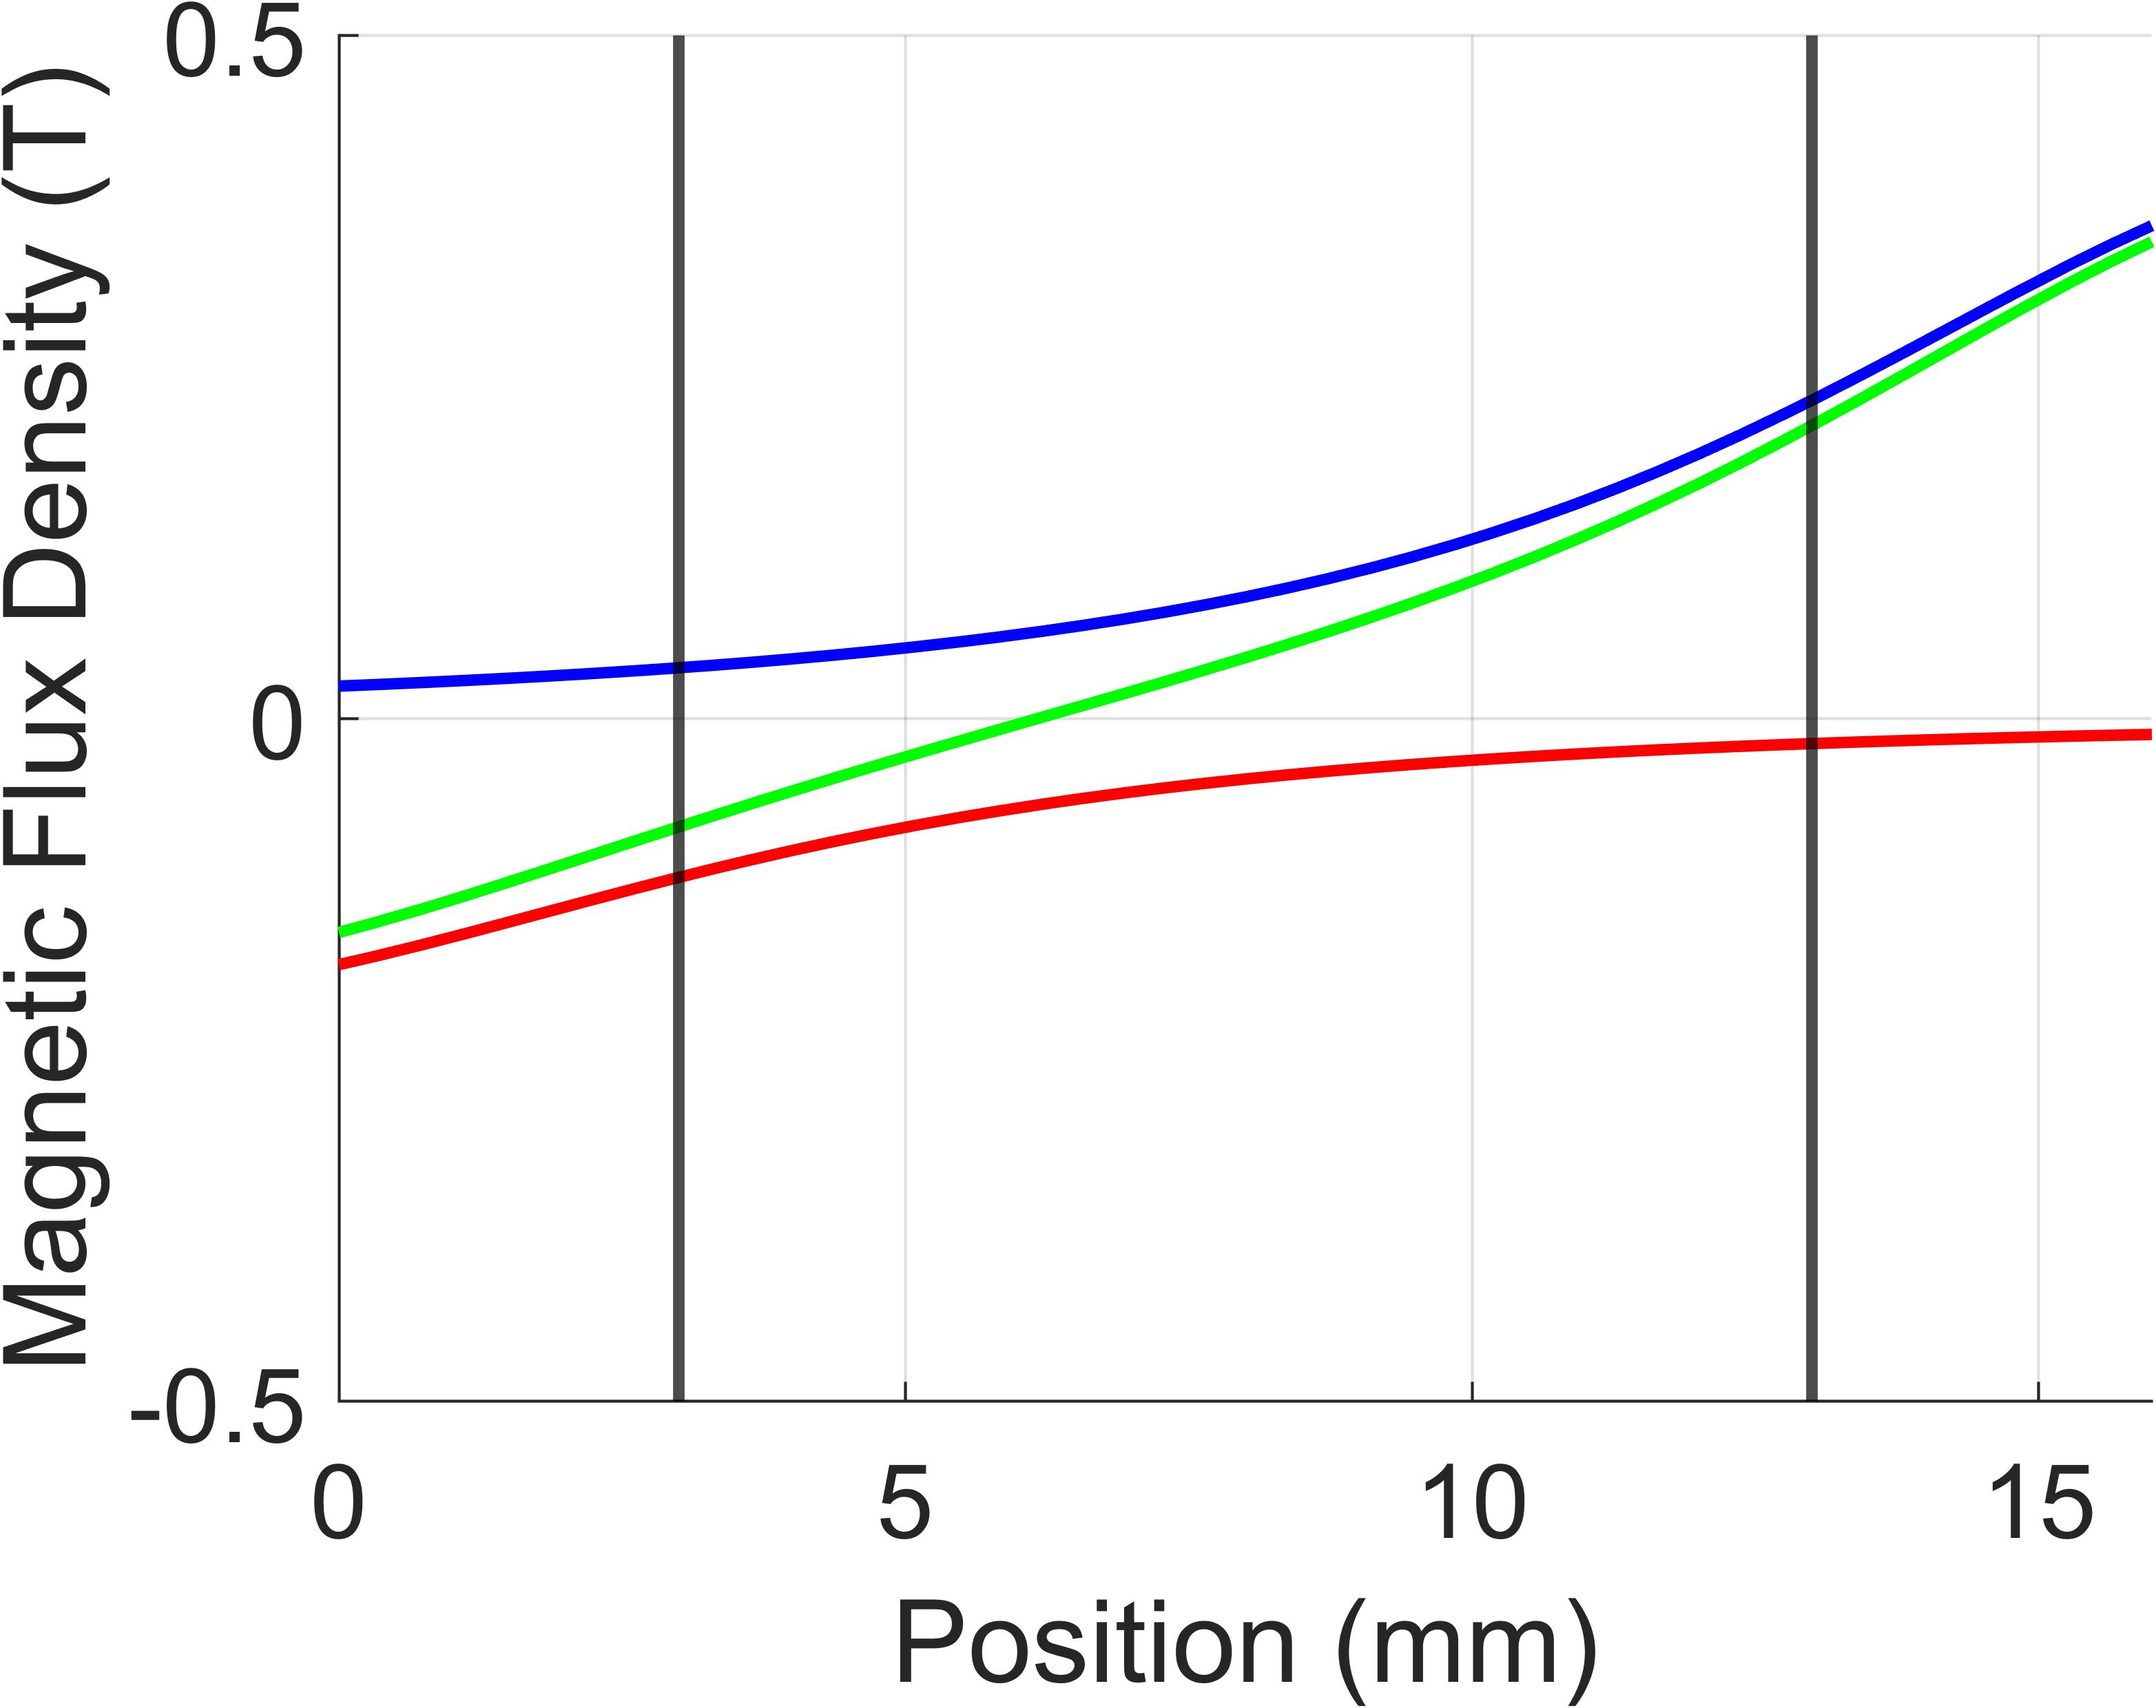
\includegraphics[width=.9\linewidth]{FluxOneTwentyDeg.jpg}
	%		\caption{\SI{120}{\degree} Phase}
	%		\label{fig:Flux120}
	%	\end{subfigure}
%	\hfill
%	\begin{subfigure}[b]{.475\textwidth}
	%		\centering
	%		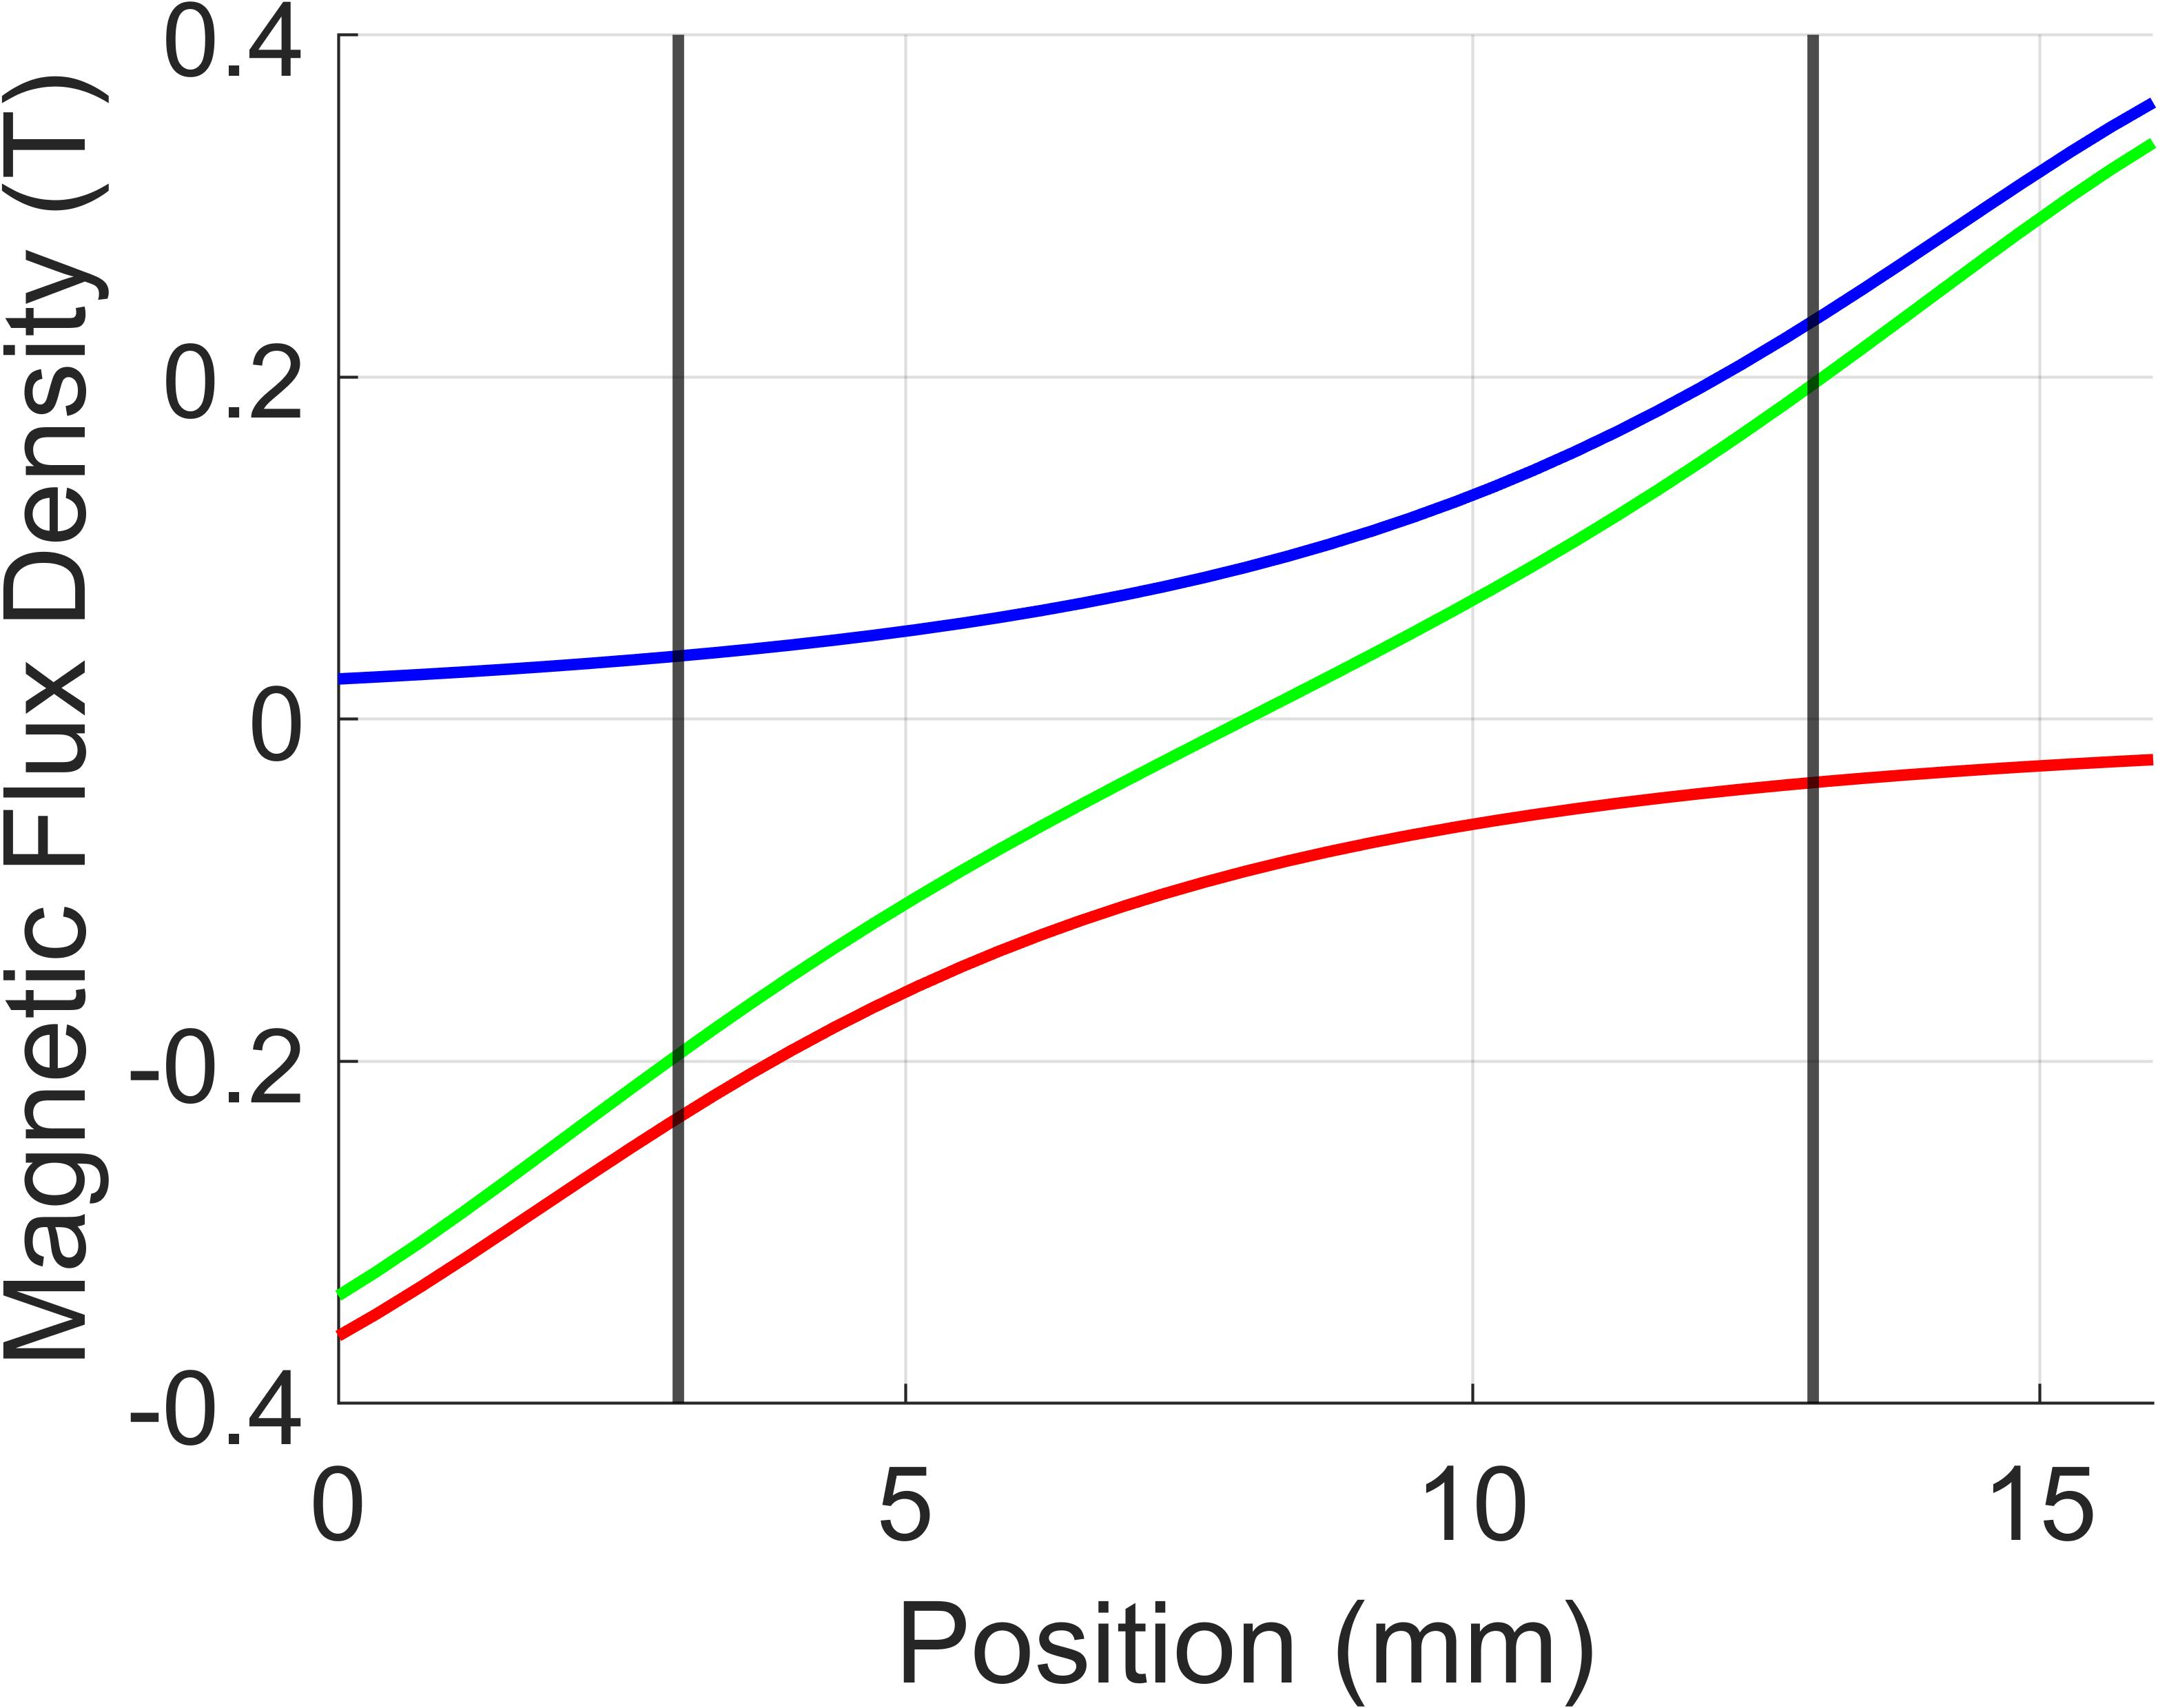
\includegraphics[width=.9\linewidth]{FluxOneEightyDeg.jpg}
	%		\caption{\SI{180}{\degree} Phase}
	%		\label{fig:Flux180}
	%	\end{subfigure}
%	\begin{subfigure}{.475\textwidth}
	%		\centering
	%		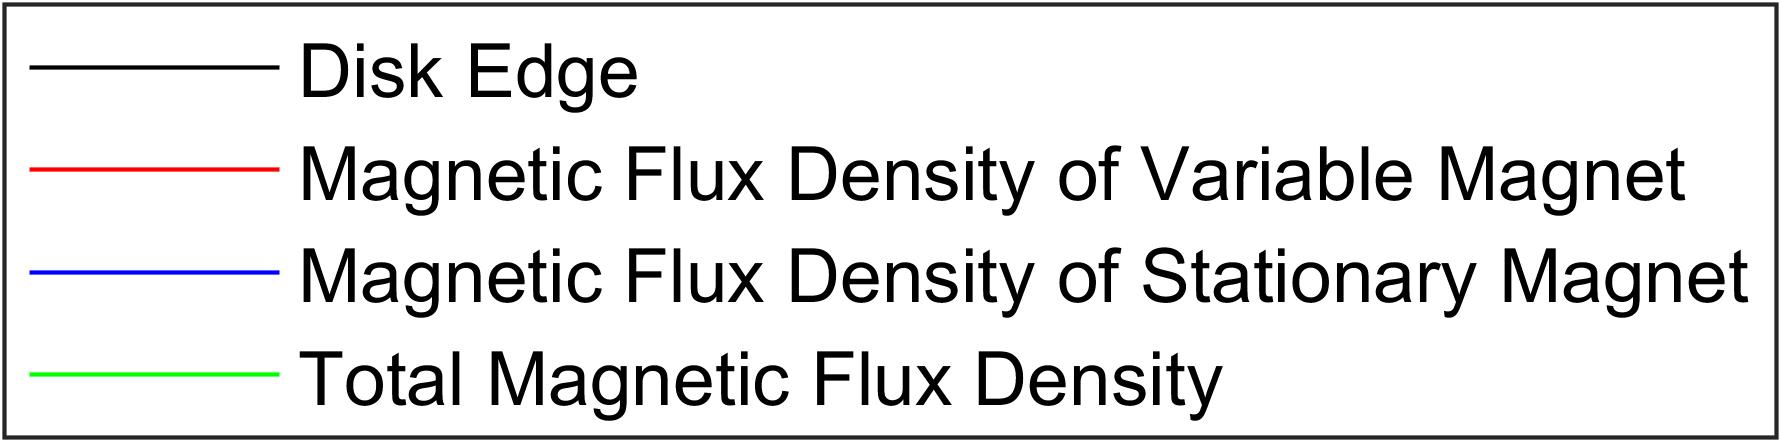
\includegraphics[width=\linewidth]{FluxLegend.jpg}
	%	\end{subfigure}
%	\caption{Flux Distribution}
%	\label{fig:Flux}
%\end{figure}
